%=============================================================================
%  Dynamic Hedge Ratio -- Pipeline Orchestration
%  dynamic_beta.py | Project Dark-Wing
%  Financial Mathematics / Time Series Analysis / Kalman_Filter
%=============================================================================
\documentclass[10pt,a4paper,twocolumn]{article}

%--- Geometry ----------------------------------------------------------------
\usepackage[a4paper,top=1.8cm,bottom=1.8cm,left=1.5cm,right=1.5cm,
            columnsep=0.7cm]{geometry}

%--- Math --------------------------------------------------------------------
\usepackage{amsmath,amssymb,amsthm,mathtools}

%--- Typography --------------------------------------------------------------
\usepackage[T1]{fontenc}
\usepackage{lmodern}
\usepackage{microtype}
\usepackage{parskip}
\setlength{\parskip}{2pt}

%--- Colours -----------------------------------------------------------------
\usepackage{xcolor}
\definecolor{codebg}{RGB}{245,247,250}
\definecolor{codeframe}{RGB}{180,195,220}
\definecolor{keyword}{RGB}{0,80,180}
\definecolor{comment}{RGB}{80,115,80}
\definecolor{string}{RGB}{160,40,20}
\definecolor{mathbluebg}{RGB}{230,240,255}
\definecolor{mathblue}{RGB}{10,60,160}
\definecolor{accent}{RGB}{25,95,195}
\definecolor{greenbg}{RGB}{230,250,232}
\definecolor{greenframe}{RGB}{50,155,70}
\definecolor{yellowbg}{RGB}{255,252,230}
\definecolor{yellowframe}{RGB}{180,150,0}
\definecolor{notebg}{RGB}{248,245,255}
\definecolor{noteframe}{RGB}{120,80,180}

%--- Code listings -----------------------------------------------------------
\usepackage{listings}
\lstdefinestyle{pythonplain}{
  language=Python,
  backgroundcolor=\color{codebg},
  frame=single,rulecolor=\color{codeframe},
  basicstyle=\ttfamily\fontsize{6.5}{8}\selectfont,
  keywordstyle=\bfseries\color{keyword},
  commentstyle=\itshape\color{comment},
  stringstyle=\color{string},
  numbers=none,breaklines=true,tabsize=2,
  showstringspaces=false,aboveskip=3pt,belowskip=3pt,
  xleftmargin=4pt,
}

%--- TikZ --------------------------------------------------------------------
\usepackage{tikz}
\usetikzlibrary{shapes.geometric,arrows.meta,positioning,calc,
                backgrounds,decorations.pathreplacing,fit}
\raggedbottom

\tikzset{
  fc_start/.style={rectangle,rounded corners=5pt,
    draw=accent,fill=accent!18,
    text width=4.4cm,align=center,
    font=\footnotesize\bfseries,
    inner sep=4pt,minimum height=0.6cm},
  fc_proc/.style={rectangle,
    draw=black!55,fill=white,
    text width=4.4cm,align=center,
    font=\footnotesize,
    inner sep=3pt,minimum height=0.58cm},
  fc_dec/.style={diamond,aspect=2.5,
    draw=accent,fill=accent!9,
    text width=2.9cm,align=center,
    font=\fontsize{6.2}{7.2}\selectfont,
    inner sep=1pt},
  fc_out/.style={rectangle,rounded corners=3pt,
    draw=greenframe,fill=greenbg,
    text width=4.4cm,align=center,
    font=\footnotesize,
    inner sep=3pt,minimum height=0.58cm},
  fc_side/.style={rectangle,
    draw=black!45,fill=yellow!10,
    text width=2.0cm,align=center,
    font=\fontsize{6.2}{7.2}\selectfont,
    inner sep=2pt,minimum height=0.52cm},
  arr/.style={-Stealth,semithick,draw=black!65},
}

%--- Boxes -------------------------------------------------------------------
\usepackage[most]{tcolorbox}
\tcbset{
  mathbox/.style={colback=mathbluebg,colframe=mathblue,
    fonttitle=\bfseries\small,title=#1,
    boxrule=0.5pt,top=3pt,bottom=3pt,left=4pt,right=4pt,
    before skip=4pt,after skip=4pt},
  exbox/.style={colback=yellowbg,colframe=yellowframe,
    fonttitle=\bfseries\small,title=#1,
    boxrule=0.5pt,top=3pt,bottom=3pt,left=4pt,right=4pt,
    before skip=4pt,after skip=4pt},
  resultbox/.style={colback=greenbg,colframe=greenframe,
    fonttitle=\bfseries\small,title=#1,
    boxrule=0.5pt,top=3pt,bottom=3pt,left=4pt,right=4pt,
    before skip=4pt,after skip=4pt},
  codebox/.style={colback=codebg,colframe=codeframe,
    fonttitle=\bfseries\small\color{accent},title=#1,
    boxrule=0.5pt,top=2pt,bottom=2pt,left=2pt,right=2pt,
    before skip=4pt,after skip=4pt},
  notebox/.style={colback=notebg,colframe=noteframe,
    fonttitle=\bfseries\small,title=#1,
    boxrule=0.5pt,top=3pt,bottom=3pt,left=4pt,right=4pt,
    before skip=4pt,after skip=4pt},
}

%--- Tables ------------------------------------------------------------------
\usepackage{booktabs,array,multirow,colortbl}

%--- Header / Footer ---------------------------------------------------------
\usepackage{fancyhdr}
\usepackage[hidelinks]{hyperref}
\pagestyle{fancy}\fancyhf{}
\fancyhead[L]{\footnotesize\textbf{DynamicBeta Orchestration --- Study Notes}}
\fancyhead[R]{\footnotesize Project Dark-Wing}
\fancyfoot[C]{\footnotesize\thepage}
\renewcommand{\headrulewidth}{0.4pt}

%--- Floats / Captions -------------------------------------------------------
\usepackage{float,caption,graphicx}
\captionsetup{font=scriptsize,labelfont=bf,skip=3pt}

%--- Section formatting ------------------------------------------------------
\usepackage{titlesec}
\titlespacing*{\section}{0pt}{7pt}{3pt}
\titlespacing*{\subsection}{0pt}{5pt}{2pt}
\titlespacing*{\subsubsection}{0pt}{3pt}{1pt}
\titleformat{\section}{\normalfont\bfseries\color{accent}}{}{0em}{}
  [{\color{accent}\titlerule[0.5pt]}]
\titleformat{\subsection}{\normalfont\bfseries\small}{}{0em}{}
\titleformat{\subsubsection}{\normalfont\itshape\small}{}{0em}{}

%--- Macros ------------------------------------------------------------------
\newcommand{\tauhl}{\tau_{\text{half-life}}}

\begin{document}

\twocolumn[{%
\begin{center}
  {\LARGE\bfseries\color{accent} Dynamic Hedge Ratio Pipeline Orchestrator}\\[5pt]
  {\large\bfseries \texttt{dynamic\_beta.py} --- Mathematical Notes \& Documentation}\\[3pt]
  {\small\itshape OLS Initialization, Kalman State Tracking, RTS Smoothing, and Z-Score Signaling}\\[3pt]
  {\small Project Dark-Wing \quad|\quad \today}
\end{center}
\vspace{4pt}
\noindent\rule{\linewidth}{0.5pt}\vspace{2pt}
\begin{quote}\small
\textbf{Abstract.}~Practical statistical arbitrage demands a cohesive execution pipeline. Rather than operating isolated models, \texttt{dynamic\_beta.py} acts as the primary orchestrator that chains several modules: static Ordinary Least Squares (OLS) initialization, Ornstein-Uhlenbeck (OU) mean-reversion analysis, Kalman Filter state tracking, RTS smoother optimization, and rolling Z-score generation. Additionally, it implements a rolling CUSUM-style variance regime-detection test to alert downstream execution modules of structural breaks in the hedge ratio. This document reviews the mathematical details of the parameter heuristics, pipeline flow, and structural break checking.
\end{quote}
\noindent\rule{\linewidth}{0.5pt}\vspace{5pt}
}]

%=============================================================================
\section{Pipeline Architecture \& Components}
%=============================================================================

In high-frequency pairs trading, estimating the dynamic hedge ratio is prone to tracking lag and noise sensitivity. The orchestrator mitigates this by layering estimation filters in sequence:
\[
  \text{OLS} \to \text{OU Half-Life} \to \text{Q/R Heuristic} \to \text{Kalman Filter}\\ \to \text{RTS Smoother} \to \text{Z-Score}
\]

Each component plays a specific role:
\begin{enumerate}\setlength\itemsep{0pt}
  \item \textbf{SpreadBuilder (OLS)}: Runs a static baseline regression to obtain initial beta ($\beta_0$) and standard residual variance.
  \item \textbf{HalfLife (OU)}: Analyzes the OLS residuals to extract the half-life of mean reversion ($\tau$). This window size is crucial for setting downstream rolling periods.
  \item \textbf{Heuristic Engine}: Dynamically sets the process noise $Q$ and measurement noise $R$ to prevent covariance collapse.
  \item \textbf{KalmanFilterPairs (Causal)}: Evaluates dynamic filtering hedge ratios $\hat{\beta}_{t|t}$ for live trading signals.
  \item \textbf{KalmanSmoother (Non-Causal)}: Performs RTS backward smoothing to produce $\hat{\beta}_{t|T}$ for historical backtest calibration.
  \item \textbf{ZScore}: Generates normalised entry/exit signals on the dynamic spread.
\end{enumerate}

%=============================================================================
\section{The Q/R Parameter Heuristic}
%=============================================================================

The performance of the Kalman Filter hinges on the ratio of the process noise covariance $Q$ to the measurement noise covariance $R$.
\begin{itemize}
  \item $Q$ too large relative to $R$: The filter overreacts to price shocks, causing the hedge ratio $\hat{\beta}_{t|t}$ to fluctuate erratically, increasing transaction costs.
  \item $R$ too large relative to $Q$: The filter ignores the time-varying nature of the relationship, converging to a static OLS model.
\end{itemize}

To provide robust initial conditions before MLE optimization, we derive a noise heuristic using the Ornstein-Uhlenbeck (OU) process properties of the spread:
\[
  d S_t = -\kappa (S_t - \theta) dt + \sigma dW_t
\]
where $\kappa$ is the speed of mean reversion, $\tauhl = \ln(2)/\kappa$, and $\sigma$ is the residual volatility.

\begin{tcolorbox}[mathbox={Q/R Noise Heuristics}]
Under the assumption that the spread follows an OU process, the process variance $Q$ of the hedge ratio scales inversely with the half-life:
\begin{equation}
  Q \approx \frac{\sigma_{\text{resid}}^2}{\tauhl}
  \label{eq:q_heuristic}
\end{equation}
where $\sigma_{\text{resid}}^2$ is the variance of the residuals of the OU process. The measurement noise covariance $R$ is initialized to the total variance of the static OLS spread:
\begin{equation}
  R \approx \text{Var}( S_t^{\text{OLS}} )
  \label{eq:r_heuristic}
\end{equation}
\end{tcolorbox}

%=============================================================================
\section{The Complete Fitting Pipeline}
%=============================================================================

The orchestrator executing \texttt{DynamicBeta.fit()} steps through the following sequence:

\subsection{Phase 1: Baseline Static Regression}
First, we run static OLS:
\[
  Y_t = \alpha_0 + \beta_0 X_t + e_t
\]
This provides the prior hedge ratio $\beta_0$. The residuals $S_t^{\text{OLS}} = Y_t - \beta_0 X_t$ form the initial spread.

\subsection{Phase 2: Half-Life Estimation}
We discretize the spread as an AR(1) process:
\[
  S_t^{\text{OLS}} - S_{t-1}^{\text{OLS}} = a + b S_{t-1}^{\text{OLS}} + \eta_t
\]
We estimate $b$ via OLS, which yields the speed of mean reversion:
\[
  \kappa = -\ln(1 + b)
\]
and the half-life of mean reversion:
\[
  \tauhl = \frac{\ln(2)}{\kappa}
\]

\subsection{Phase 3: Kalman State Update}
We initialize the Kalman Filter with $\hat{\beta}_{0|0} = \beta_0$ and $P_{0|0} = 1000.0$. We set $Q$ and $R$ from the heuristics in Eq.~\eqref{eq:q_heuristic} and Eq.~\eqref{eq:r_heuristic}. We run the filter over the log prices, yielding the filtered states:
\[
  \hat{\beta}_{t|t}, \quad P_{t|t}, \quad \text{and} \quad S_t = Y_t - \hat{\beta}_{t|t} X_t
\]

\subsection{Phase 4: RTS Smoothing}
For backtest calibration, we run the RTS backward smoother to obtain:
\[
  \hat{\beta}_{t|T}, \quad P_{t|T}, \quad \text{and} \quad S_t^{\text{smooth}} = Y_t - \hat{\beta}_{t|T} X_t
\]

\subsection{Phase 5: Signal Normalization}
The dynamic spread $S_t$ is normalized using a rolling Z-score with window size $W = 2\tauhl$:
\[
  Z_t = \frac{S_t - \mu_{\text{roll}}(S_t, W)}{\sigma_{\text{roll}}(S_t, W)}
\]
The strategy generates buy/sell signals on $Z_t$.

%=============================================================================
\section{Regime Detection Algorithm}
%=============================================================================

In statistical arbitrage, a critical risk is cointegration breakdown (the assets diverge permanently due to structural reasons). This manifests as a level shift in $\beta_t$. We detect this via a rolling CUSUM-style test on the hedge ratio.

\begin{tcolorbox}[mathbox={Structural Break Detection}]
Let $\mu_{\text{global}}$ be the mean of $\beta_t$ over the entire historical window. For each timestep $t$, we compute the rolling average $\mu_{\text{roll}}(t, W)$ and rolling standard deviation $\sigma_{\text{roll}}(t, W)$ over a lookback window $W = 126$ (6 months). A regime break is flagged if the deviation exceeds a statistical threshold:
\begin{equation}
  \left| \mu_{\text{roll}}(t, W) - \mu_{\text{global}} \right| > K \cdot \sigma_{\text{roll}}(t, W)
\end{equation}
where $K$ is the sensitivity parameter (default $K = 2.0$).
\end{tcolorbox}

When a regime break is flagged, it signals that the historical cointegration relation has broken down, and trade execution should reduce position sizes or halt entries.

%=============================================================================
\section{Worked Numerical Example}
%=============================================================================

\begin{tcolorbox}[exbox={Pipeline Initialization Example}]
Let $Y$ and $X$ be log-prices with $N=252$ days.
\begin{enumerate}\setlength\itemsep{0pt}
  \item \textbf{OLS Result}: $\beta_0 = 1.25$, $\text{Var}(S^{\text{OLS}}) = 0.04$.
  \item \textbf{OU Fit}: Speed of mean reversion $\kappa = 0.055$ per day.
  \item \textbf{Half-life}: $\tauhl = \ln(2)/0.055 = 12.6 \approx 13$ days.
  \item \textbf{OU Residual Variance}: $\sigma_{\text{resid}}^2 = 0.0013$.
\end{enumerate}
\end{tcolorbox}

Using these estimates, the orchestrator sets:
\[
  R = 0.04
\]
\[
  Q = \frac{0.0013}{13} = 1.0 \times 10^{-4}
\]
The Kalman Filter is initialized with:
\[
  \hat{\beta}_{0|0} = 1.25, \quad P_{0|0} = 1000.0
\]
The rolling Z-score window is set to:
\[
  W = 2 \times 13 = 26 \text{ days}
\]
This prevents arbitrary window selection and links signal generation directly to the underlying mean-reversion speed.\\
\vspace{1 cm}

%=============================================================================
\section{Class Structure \& Flowchart}
%=============================================================================
\begin{center}
  \begin{figure}[H]
    \centering
  \resizebox{\columnwidth}{!}{%
  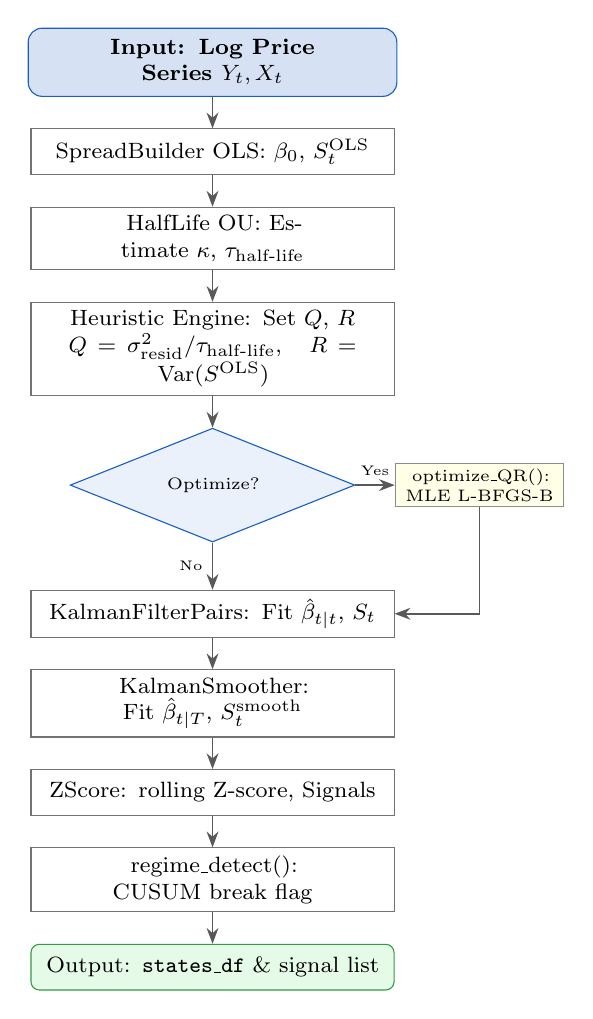
\begin{tikzpicture}[node distance=0.4cm,every node/.style={font=\scriptsize}]
    \node (in) [fc_start] {Input: Log Price Series $Y_t, X_t$};
    \node (ols) [fc_proc,below=of in] {SpreadBuilder OLS: $\beta_0$, $S_t^{\text{OLS}}$};
    \node (hl) [fc_proc,below=of ols] {HalfLife OU: Estimate $\kappa$, $\tauhl$};
    \node (heur) [fc_proc,below=of hl] {Heuristic Engine: Set $Q$, $R$\\
      $Q = \sigma_{\text{resid}}^2/\tauhl, \quad R = \text{Var}(S^{\text{OLS}})$};
      \node (mle) [fc_dec,below=of heur] {Optimize?};
      \node (opt) [fc_side,right=0.5cm of mle] {optimize\_QR():\\ MLE L-BFGS-B};
    \node (kf) [fc_proc,below=0.6cm of mle] {KalmanFilterPairs: Fit $\hat{\beta}_{t|t}$, $S_t$};
    \node (sm) [fc_proc,below=of kf] {KalmanSmoother: Fit $\hat{\beta}_{t|T}$, $S_t^{\text{smooth}}$};
    \node (zs) [fc_proc,below=of sm] {ZScore: rolling Z-score, Signals};
    \node (reg) [fc_proc,below=of zs] {regime\_detect(): CUSUM break flag};
    \node (out) [fc_out,below=of reg] {Output: \texttt{states\_df} \& signal list};
    
    \draw[arr] (in) -- (ols);
    \draw[arr] (ols) -- (hl);
    \draw[arr] (hl) -- (heur);
    \draw[arr] (heur) -- (mle);
    \draw[arr] (mle) -- node[left,font=\tiny]{No} (kf);
    \draw[arr] (mle) -- node[above,font=\tiny]{Yes} (opt);
    \draw[arr] (opt) |- (kf);
    \draw[arr] (kf) -- (sm);
    \draw[arr] (sm) -- (zs);
    \draw[arr] (zs) -- (reg);
    \draw[arr] (reg) -- (out);
  \end{tikzpicture}
  }
  \caption{Process flow of the \texttt{DynamicBeta} pipeline.}
  \end{figure}
\end{center}

%=============================================================================
\section{Python Implementation Snippets}
%=============================================================================

\begin{tcolorbox}[codebox={\texttt{dynamic\_beta.py} Main Architecture}]
\begin{lstlisting}[style=pythonplain]
class DynamicBeta:
    def __init__(self, y, x, Q=None, R=None, P_init=1000.0,
                 beta_init=None, optimize=False,
                 half_life_window=252, entry_z=2.0,
                 exit_z=0.5, stop_z=3.5, run_smoother=True):
        self._y = y; self._x = x
        self.P_init = P_init
        self.optimize = optimize
        self.entry_z = entry_z; self.exit_z = exit_z; self.stop_z = stop_z
        self.run_smoother_flag = run_smoother
        
        # Step 1: OLS baseline
        self._sb = SpreadBuilder(y=self._y, x=self._x, mode="ols").build()
        ols_beta = self._sb.get_beta()
        self._ols_spread = self._sb.spread_series()
        
        # Step 2: Half-Life
        _hl = HalfLife(self._ols_spread).estimate()
        self._tau = _hl.half_life_days
        
        # Step 3: Heuristics
        _ou_resid_var = np.var(_hl.get_ou_residuals())
        self._Q = Q if Q is not None else max(1e-8, _ou_resid_var/self._tau)
        self._R = R if R is not None else np.var(self._ols_spread.values)
        self._beta_init = beta_init if beta_init is not None else ols_beta

    def fit(self):
        self._kf = KalmanFilterPairs(Q=self._Q, R=self._R,
                                     beta_init=self._beta_init, P_init=self.P_init)
        if self.optimize:
            self._kf.optimize_QR(self._y, self._x)
        self._states_df = self._kf.filter(self._y, self._x)
        
        if self.run_smoother_flag:
            self._ks = KalmanSmoother(self._kf)
            self._ks.smooth()
            self._states_df["smoothed_beta"] = self._ks._smoothed_beta
            self._states_df["smoothed_spread"] = self._ks.smoothed_spread().values
            
        kalman_spread = self._kf.spread_series()
        zs_window = max(10, int(self._tau * 2))
        self._zscore = ZScore(kalman_spread, window=zs_window, mode="rolling",
                              entry_z=self.entry_z, exit_z=self.exit_z, stop_z=self.stop_z)
        self._zscore.compute()
        self._zscore.generate_signals()
        
        self._states_df["zscore"] = self._zscore.zscore_series().values
        self._states_df["signal"] = self._zscore.signal_series().values
        self._fitted = True
        return self._states_df
\end{lstlisting}
\end{tcolorbox}

%=============================================================================
\section{The EM Algorithm for Variance Tuning}
%=============================================================================

While direct Maximization of Log-Likelihood (MLE) using Scipy's \texttt{L-BFGS-B} is robust, the Expectation-Maximization (EM) algorithm provides an elegant, derivative-free iterative framework for estimating the noise covariances $Q$ and $R$. 

The EM algorithm treats the hidden hedge ratios $\beta_{1:T}$ as latent variables and alternates between:
\begin{itemize}
  \item \textbf{E-step}: Run the Kalman Filter and RTS Smoother using current parameter guesses $Q^{(j)}, R^{(j)}$ to compute the smoothed state expectations $\mathbb{E}[\beta_t \mid \mathcal{F}_T] = \hat{\beta}_{t|T}$ and covariances $P_{t|T}$.
  \item \textbf{M-step}: Maximize the expected log-likelihood of the complete data relative to $Q$ and $R$.
\end{itemize}

\begin{tcolorbox}[mathbox={EM Update Equations}]
The updated process variance $Q^{(j+1)}$ and measurement variance $R^{(j+1)}$ are computed from the smoothed states as:
\begin{equation}
  Q^{(j+1)} = \frac{1}{T-1} \sum_{t=2}^T \left[ (\hat{\beta}_{t|T} - \hat{\beta}_{t-1|T})^2 + P_{t|T} + P_{t-1|T} - 2 P_{t,t-1|T} \right]
  \label{eq:Q_em}
\end{equation}
\begin{equation}
  R^{(j+1)} = \frac{1}{T} \sum_{t=1}^T \left[ (Y_t - \hat{\beta}_{t|T} X_t)^2 + X_t^2 P_{t|T} \right]
  \label{eq:R_em}
\end{equation}
where the lag-1 covariance is obtained via:
\[
  P_{t,t-1|T} = P_{t|T}\,\Xi_{t-1}
\]
\end{tcolorbox}
The EM algorithm converges monotonically to a local maximum of the likelihood function. It is particularly stable when the initial parameter guesses derived from the OU heuristics in Eq.~\eqref{eq:q_heuristic} and Eq.~\eqref{eq:r_heuristic} are used as starting values.

%=============================================================================
\section{Signal Threshold Optimization}
%=============================================================================

In the ZScore normalization phase, setting the entry threshold $Z_{\text{entry}}$ (e.g., $2.0$) and exit threshold $Z_{\text{exit}}$ (e.g., $0.5$) determines the trade frequency and win rate. 

Under the assumption of a stationary de-meaned Gaussian spread $S_t \sim \mathcal{N}(0, \sigma^2)$, the probability that the spread deviates beyond $Z_{\text{entry}}$ standard deviations is:
\[
  P(|Z| > Z_{\text{entry}}) = 2 \left( 1 - \Phi(Z_{\text{entry}}) \right)
\]
For $Z_{\text{entry}} = 2.0$, this probability is approximately $4.56\%$. The expected time between entry signals is proportional to the half-life:
\begin{tcolorbox}[mathbox={Expected Trade Frequency}]
\begin{equation}
  \mathbb{E}[T_{\text{wait}}] \propto \frac{\tauhl}{P(|Z| > Z_{\text{entry}})}
\end{equation}
If the assets' half-life $\tauhl$ is short, the spread reverts rapidly, allowing for frequent round-trip trades. If $\tauhl$ is long, the trade frequency drops, and capital is locked up for longer durations, requiring wider entry thresholds to ensure adequate margin of safety.
\end{tcolorbox}

%=============================================================================
\section{Interview Preparation}
%=============================================================================

\begin{tcolorbox}[exbox={Key Pipeline Orchestration Questions}]
\begin{enumerate}\setlength\itemsep{1pt}
  \item \textbf{Why do we use OLS regression to initialize the Kalman Filter?}\\
    The Kalman Filter requires a prior state mean $\beta_{0|0}$. Using OLS provides a statistically optimal prior baseline, accelerating the filter convergence.
  \item \textbf{How does the OU half-life help size the Z-score lookback window?}\\
    The half-life represents the average duration of a deviation. Sizing the window to $2\tau$ ensures the rolling mean and standard deviation capture both the deviation and reversion phases.
  \item \textbf{What is the financial danger of ignoring a regime break?}\\
    If cointegration breaks down, the spread becomes a random walk. The Z-score will remain wide, triggering continuous buy/sell orders that result in large drawdowns.
  \item \textbf{Why run the RTS smoother in backtests but not in production?}\\
    The RTS smoother utilizes future information to refine past estimates. This is optimal for historical parameter calibration but impossible for real-time execution.
\end{enumerate}
\tcblower
\textbf{Variance break heuristic}: A rapid drop in the Kalman variance $P_{t|t}$ suggests the model has converged on a stable relation.
\end{tcolorbox}

%=============================================================================
\section{Pipeline Position}
%=============================================================================

\begin{center}{\small
\begin{tabular}{@{}clp{2.5cm}@{}}
\toprule Step & Module & Output\\\midrule
5a & \texttt{spread\_builder.py} & Initial Spread\\
5b & \texttt{half\_life.py} & $\tauhl$ windows\\
6a & \texttt{kalman\_filter.py} & Filter recursion\\
6b & \texttt{smoother.py} & Backward smoothing\\
\textbf{6c} & \textbf{\texttt{dynamic\_beta.py}} & Full Pipeline orchestrator\\
7 & \texttt{kalman\_forecast.py} & Spread projections\\
8 & \texttt{signal/pair\_signal.py} & Entry/exit logic\\
\bottomrule
\end{tabular}
}\end{center}

\end{document}
